\chapter{Notions d'estimation}
\section{Rappels des cours de 1A}
\subsection{Espace de Hilbert}
\begin{definition}{Espaces de Hilbert}{Espaces de Hilbert}
    Un espace de Hilbert est un \textbf{espace préhilbertien complet}, c'est à dire un \textbf{espace de Banach} dont la norme $||.||$ découle d'un \textbf{produit scalaire} ou \textbf{hermitien} par la formule suivante :
    \begin{equation}
        ||x|| = \sqrt{\langle x,x \rangle}
    \end{equation}
\end{definition}
\begin{definition}{Espaces de Banach}{Espaces de Banach}
    Un espace de Banach est un \textbf{espace vectoriel complet et normé} sur un sous corps $\mathbb{K}$ de $\mathbb{C}$ ($\mathbb{R}$ ou $\mathbb{C}$), peut importe la norme.
\end{definition}
\noindent \textbf{En d'autres termes, un espace de Hilbert est un espace vectoriel complet muni d'une norme définie par un produit scalaire.}
\subsection{Espace Lp}
\begin{definition}{Espaces $L^{p}[a,b]$}{Espaces Lp}
    Espace vectoriel des fonctions $p$ intégrables au sens de \textbf{Lebesgue} sur $[a,b]$. i.e.
    \begin{equation}
        \int_{a}^{b}{|f(t)|^{p}dt} 
    \end{equation}
    converge, avec la norme $L^{p}$: 
    \begin{equation}
        ||f||_{p} = \sqrt[\frac{1}{p}]{\int_{a}^{b}{|f(t)|^{p}dt}}
    \end{equation}
\end{definition}
\newpage
\subsection{Précisions}
\begin{definition}{Espace vectoriel normé}{Espace vectoriel normé}
    Un K-espace vectoriel $E$ est dit normé si il est muni d'une norme, c'est-à-dire d'une application $\mathcal{N} : E \rightarrow \mathbb{R}^{+}$ qui satisfait les conditions suivantes :
    \begin{itemize}
        \item \textbf{Séparation}
        \begin{equation}
            \forall x \in E, \mathcal{N}(x)=0 \implies x = 0_{E}  
        \end{equation} 
        \item \textbf{Homogénéité}
        \begin{equation}
            \forall (x,\lambda) \in E \times \mathbb{R}, \mathcal{N}(\lambda x) = |\lambda|\mathcal{N}(x)
        \end{equation} 
        \item \textbf{Sous-additivité (inégalité triangulaire)}
        \begin{equation}
            \forall (x,y) \in E^{2}, \mathcal{N}(x+y) < \mathcal{N}(x)\mathcal{N}(y)
        \end{equation} 
    \end{itemize}
\end{definition}
\begin{definition}{Espace métrique complet}{Espace métrique complet}
    Un espace métrique $(E,d)$ est dit complet si toute suite de Cauchy \footnote{
        Suite qui vérifie le critère de Cauchy, c'est-à-dire que les éléments de la suite se rapprochent uniformément entre-eux à l'infini, i.e. 
        \begin{equation}
            \forall \epsilon > 0, \exists (n_{0},p_{0}) \in \mathbb{N}^{2}, \forall n > n_{0}, \forall p > p_{0}, d(x_{n}, x_{p}) < \epsilon   
        \end{equation}
     } 
     converge dans ce même espace, c'est-à-dire :
    \begin{equation}
        \forall n \in \mathbb{N}, (x_{n})_{n \in \mathbb{N}} \in E, x_{n} \longrightarrow l \in E
    \end{equation}
\end{definition}
\begin{definition}{Espace métrique}{Espace métrique}
    On note $(E,d)$ un espace métrique ($E$ ensemble et $d$ la distance définie pour tout éléments de $E$). C'est un espace vectoriel au sein duquel la notion de distance est bien définie pour tout éléments de $E$. L'application $d$ satisfait les conditions suivantes :
    \begin{itemize}
        \item \textbf{Symétrie}
        \begin{equation}
            \forall (x,y) \in E^{2}, d(x,y) = d(y,x)
        \end{equation} 
        \item \textbf{Séparation}
        \begin{equation}
            \forall (x,y) \in E^{2}, d(x,y) = 0 \Longleftrightarrow x = y
        \end{equation} 
        \item \textbf{Inégalité triangulaire}
        \begin{equation}
            \forall (x,y,z) \in E^{3}, d(x,y) < d(x,z) + d(z,y)
        \end{equation} 
    \end{itemize}
\end{definition}
\newpage
\subsection{Probabilités}
\begin{definition}{Espaces probabilisé}{Espaces probabilisé}
    Un espace probabilisé est constitué d'un \textbf{espace probabilisable} et d'une \textbf{mesure de probabilité}, noté $(\Omega, \mathcal{A}, \mathbb{P})$ avec : \newline
    \begin{itemize}
        \item $\Omega$ : l'univers, l'espace des observations ou espace des évènements élémentaires
        \item $\mathcal{A}$ est une \textbf{tribu} sur $\Omega$
        \item $\mathbb{P}$ : mesure de probabilité \newline
    \end{itemize}
    \noindent tel que $\mathbb{P}(\Omega)=1$ et $\forall A \in \mathcal{A}$, $\mathbb{P}(A)$ est appelé \textit{probabilité de l'évènement $A$}
\end{definition}
\begin{definition}{Espaces probabilisables}{Espaces probabilisables}
    Un espace probabilisable est noté $(\Omega, \mathcal{A})$, il est constitué de \textbf{l'univers} et de la \textbf{tribu} de cet univers.
\end{definition}
\begin{definition}{Mesure de probabilité}{Mesure de probabilité}
   La mesure de probabilité est définie par l'application $\mathbb{P} : \Omega \longrightarrow [0;1]$ telle que :
   \begin{itemize}
    \item $\mathbb{P}(\Omega) = 1$ 
    \item $\mathbb{P}(\{\}) = 0$
    \item \textbf{$\sigma$-additivité} : $\forall $ collection dénombrable $\{ A_{i} \}$ d'ensemble disjoints :
    \begin{equation}
        \mathbb{P}(\bigcup_{I \in \mathcal{I}} A_i) = \sum_{I \in \mathcal{I}} \mathbb{P}(A_{i})
    \end{equation}
   \end{itemize}
\end{definition}
\subsection{Schématiquement}
\begin{center}
    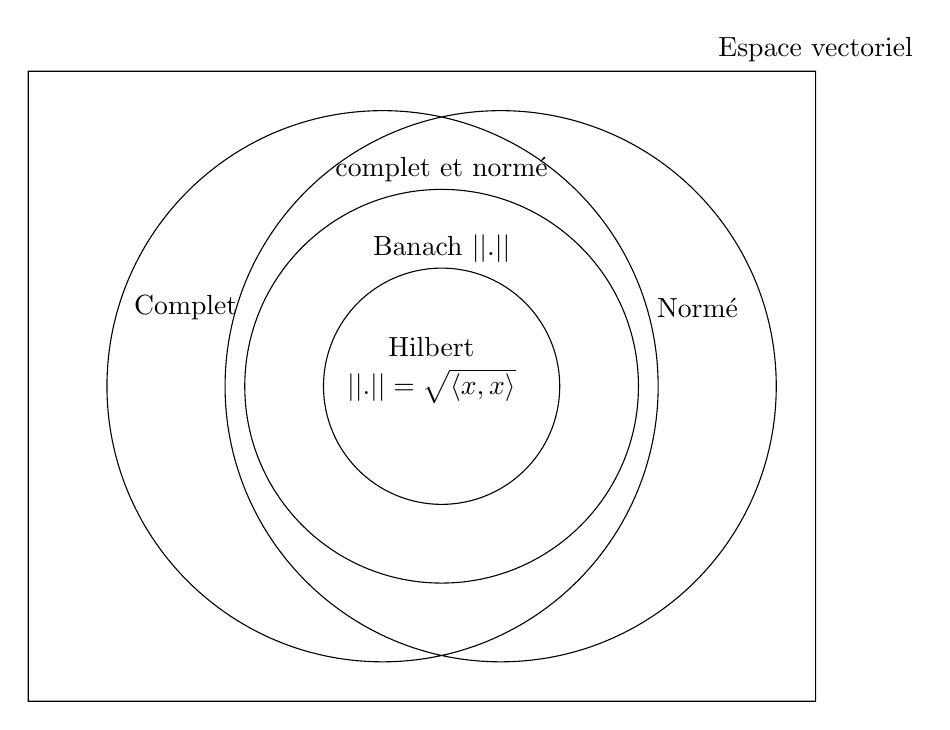
\begin{tikzpicture}[fill=red]
        \centering
        % outline
        \draw (-0.5,-1) circle (3.5) (0,1)  node at (-3,0) {Complet}
              (1,-1) circle (3.5) (1,1)  node  at (3.5,0) {Normé}
              (1,-1) circle (0) (1,0)  node  at (0.25,1.75) {complet et normé}
              (0.25,-1) circle (2.5) (1,1)  node at (0.25,0.75) {Banach $||.||$}
              (0.25,-1) circle (1.5) (1,0)  node at (0.12,-0.5) {Hilbert}
              (0.25,-1) circle (0) (1,0)  node at (0.12,-1)  {$||.|| = \sqrt{\langle x,x \rangle}$}
              (-5,-5) rectangle (5,3) node [text=black,above] {Espace vectoriel};
    \end{tikzpicture}
\end{center}
\newpage
\section{Estimation}
\subsection{Notions et définitions de base}
\noindent On cherche à reconstituer un signal $\underline{x}$ ou $\underline{\theta}$ à partir de son observation, le vecteur $\underline{y}$. On cherche alors une fonction $\widehat{\theta}$ tel que $x \circ y = \widehat{\theta}(\underline{y})$ soit la meilleure estimation de $\underline{\theta}$. \newline

\noindent Mathématiquement, on a : 
\[ \underline{\theta} = 
\begin{bmatrix}
    \theta_{0} & \theta_{1} & ... & \theta_{n} 
\end{bmatrix}
, (\theta_{i})_{i \in \mathbb{N}} \in G
\]
\[ \underline{y} = 
\begin{bmatrix}
    y_{0} & y_{1} & ... & y_{n} 
\end{bmatrix}
, (y_{i})_{i \in \mathbb{N}} \in F
\]
Avec :
\begin{itemize}
    \item $\underline{\theta}$ : \textbf{paramètre décisionnel} \newline
    \item $\underline{y}$ : \textbf{vecteur d'observation} \newline
    \item $(\theta_{i})_{i \in \mathbb{N}}$, $(y_{i})_{i \in \mathbb{N}}$ : \textbf{variables aléatoires} de $G$ et $F$ \newline
    \item $(G,\mathcal{G})$ et $(F,\mathcal{F})$ sont des espaces probabilisables \newline
\end{itemize}
\noindent \textbf{Estimateur} \newline
\noindent Pour un \textbf{estimateur $\widehat{\theta}$}, le meilleur estimateur (ou filtre) de $\theta$ est donc l'application $\widehat{\theta}$:
\begin{equation}
    \large
    \tcbhighmath[fuzzy halo=0.5mm with electricultramarine!35!electricultramarine,arc=2pt,
    boxrule=0pt,frame hidden]{ 
        \widehat{\theta} : F \longrightarrow G, \\ \widehat{\theta} \circ y = \widehat{\theta}(\underline{y}) \in \mathcal{M}(F,G)
     } \nonumber
    \normalsize
\end{equation}
Avec $\mathcal{M}(F,G)$ l'ensemble des applications de $F$ dans $G$. \newline

\noindent \textbf{Densité de probabilité conditionnelle} \newline
\noindent $(\Omega, \epsilon, P)$ est un espace probabilisé qui modélise l'expérience aléatoire (signaux aléatoires rencontrés) \newline
\noindent $\underline{y}$ est le vecteur d'observation qui admet une \textbf{densité} par rapport à $F$, de \textbf{mesure canonique}\footnote{Mesure canonique que l'on prend comme mesure de Lebesgue} $\nu$, tandis que $\widehat{\theta}(\underline{y})$ est une VA à valeurs dans $G$, alors la \textbf{densité de probabilité conditionnelle de $\underline{y}$ sachant $\theta$ } s'exprime sous la forme :
\begin{equation}
    \large
    \tcbhighmath[fuzzy halo=0.5mm with electricultramarine!35!electricultramarine,arc=2pt,
    boxrule=0pt,frame hidden]{ 
        f_{\underline{y}|\theta}(\underline{\nu}|\theta), \forall \nu \in F
     } \nonumber
    \normalsize
\end{equation}
\textbf{Fonction de perte ou de coût} : application $L$ telle que :
\begin{equation}
    L : G \times G \longrightarrow \mathbb{R}, (\theta_{1},\theta_{2}) \mapsto L[\theta_{1},\theta_{2}] \nonumber
\end{equation}
Pour un estimateur $\widehat{\theta}$ et $\nu \in F$ donnés,  $L[\widehat{\theta}(\underline{\nu}), \theta]$ représente le \textbf{coût de la décision} $\widehat{\theta}(\nu)$ quand la vraie valeur du paramètre décisionnel est $\theta$. Ce coût est généralement arbitraire. \newline
\textbf{Fonction de risque}
\begin{equation}
    \mathcal{R}(\widehat{\theta},\theta) = E[L(\widehat{\theta}(\underline{y}),\theta)|\theta] = \int_{F}{L[\widehat{\theta}(\underline{\nu}), \theta]f_{\underline{y}|\theta}(\underline{\nu}|\theta)}{d\underline{\nu}} \nonumber
\end{equation}
\newpage
\subsection{Point de vu Bayésien et non Bayésien}
\begin{itemize}
    \item \textbf{Non Bayésien} : $\theta$ est supposé déterministe, c'est à dire qu'il obéit à des lois non probabilistes \newline
    \item \textbf{Bayésien} : $\theta$ est supposé aléatoire et de loi connue \newline
    \item \textbf{Paramétrique} : $\theta$ est aléatoire et de loi connue (i.e. Bayésien sans supposition) \newline
    \item \textbf{Non Paramétrique} : $\theta$ est aléatoire et de loi inconnue. \newline
\end{itemize}
\noindent Le point de vu \textbf{fréquentiste}, i.e. non paramétrique ne sera étudié dans le cadre de ce cours. Le point de vu Bayésien permet d'introduire d'autres notions telles que : \newline

\noindent \textbf{Risque moyen} \newline
\noindent pour une \textbf{densité de probabilité a fortiori $f_{\theta}(u)$} du paramètre décisionnel, le risque moyen s'exprime sous la forme :
\begin{equation}
    \overline{R}(\widehat{\theta}) = E[R(\widehat{\theta}), \theta] = \int_{G}{R(\widehat{\theta},u)}f_{\theta}(u)du = \int_{F}{H_{c}(\underline{\nu})f_{y}(\underline{\nu})}d\underline{\nu}
\end{equation}
Avec
\begin{equation}
    H_{c}(\underline{\nu}) =  \int_{G}{L[\widehat{\theta}(\underline{\nu}), u]f_{\theta | y}(u|\underline{\nu})}du = E\{L[\widehat{\theta}(\underline{y}),\theta]|\underline{y}=\underline{\nu}\}
\end{equation}
La ddp conditionnelle $f_{\theta | y}(u|\underline{\nu})$ devient la \textbf{densité de probabilité a posteriori} et la loi de $\underline{y}$ est \textbf{l'evidence}